\section{Rolling-Window Fair Value Model}

\subsection*{Motivation}

The main report estimates CDX IG fair value using a static OLS model: a single
set of coefficients is estimated on the training set and applied unchanged to
the full sample. This implicitly assumes that the relationship between CDX IG
and its drivers (\(\Delta VIX\), \(\Delta S\&P\), \(\Delta UST10\),
\(\Delta USYC\), \(\Delta SOFR\)) is time-invariant.

Given the evidence of regime changes documented in the main report
(Sections~5--7), this assumption may be restrictive. An alternative is a
rolling-window approach in which the OLS coefficients are re-estimated at each
date using only the most recent \(N\) observations. This allows the model to
adapt to evolving market regimes but introduces additional estimation noise and
reduces the effective sample available for each regression.

\subsection*{Specification}

The same five-variable model from the main report is re-estimated using a
trailing 180-day (approximately 6-month) rolling window:
\[
\Delta CDXIG_t = \alpha_t + \gamma_{1,t} \Delta VIX_t + \gamma_{2,t} \Delta S\&P_t
  + \gamma_{3,t} \Delta UST10_t + \gamma_{4,t} \Delta USYC_t
  + \gamma_{5,t} \Delta SOFR_t + u_t
\]
where the subscript \(t\) on the coefficients indicates that they are estimated
on the window \([t - 180, \, t - 1]\) and applied to predict the change at
date \(t\). This is a strictly out-of-sample exercise: each day's prediction
uses only past information.

\subsection*{Results}

\begin{itemize}
  \item \textbf{Rolling model \(R^2 \approx 0.496\)} on daily changes, compared
    with \(R^2 \approx 0.698\) for the static model's out-of-sample test set.
  \item \textbf{Rolling model RMSE \(\approx 2.28\)}, compared with
    \(\approx 1.60\) for the static model.
  \item Number of evaluated observations: 1\,010 (after the initial 180-day
    burn-in period).
\end{itemize}

The static model outperforms the rolling model on both \(R^2\) and RMSE. This
is consistent with two factors:
\begin{enumerate}
  \item The static model benefits from estimating coefficients on a larger
    training sample (approximately 1\,040 observations vs.\ 180 at each rolling
    step), which reduces parameter estimation error.
  \item The relationships between CDX IG and its macro drivers, while exhibiting
    regime variation, are sufficiently stable over this sample that a single
    coefficient set captures the dominant dynamics effectively.
\end{enumerate}

However, the rolling model has the advantage of being fully adaptive: it does
not require a fixed train/test split and can be deployed in real time. In
environments where the macro regime shifts more rapidly (e.g.\ the 2020 COVID
episode or the 2022 tightening cycle), a rolling approach may produce more
timely fair-value estimates despite higher aggregate error.

\begin{figure}[H]
  \centering
  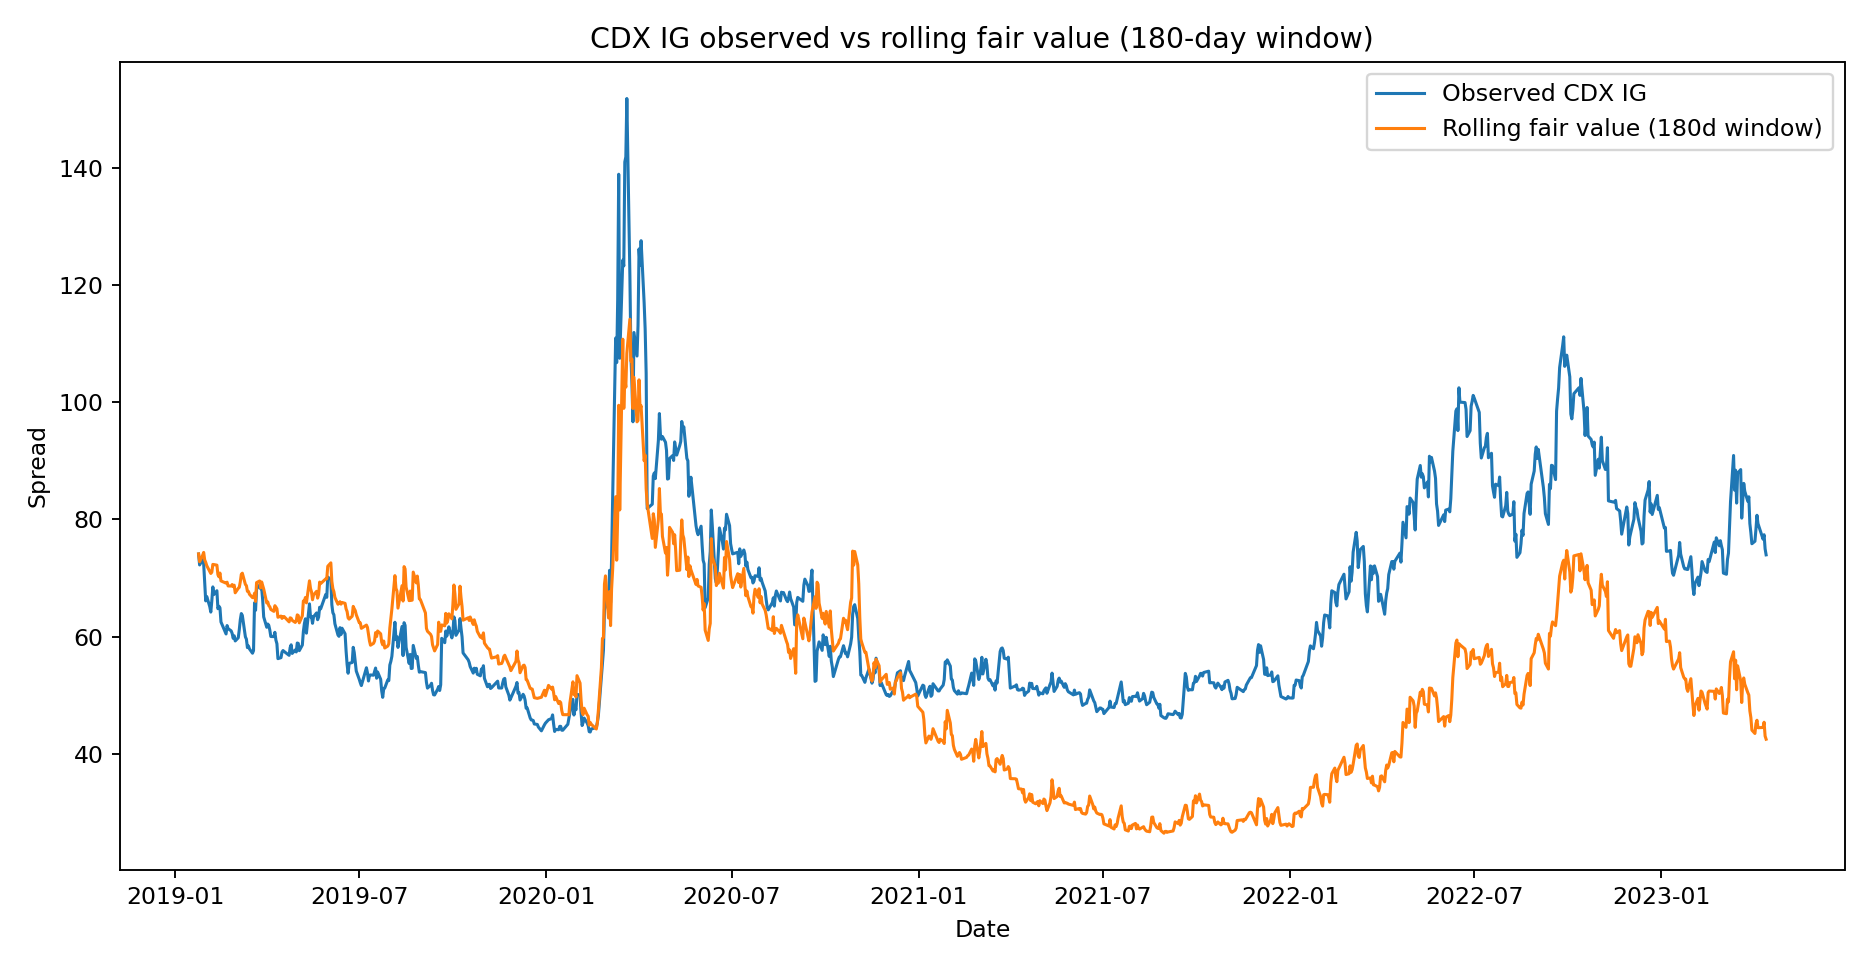
\includegraphics[width=\textwidth]{../../../output/figures/CDX_IG_rolling_fair_value.png}
  \caption{Observed CDX IG vs rolling fair-value level (180-day estimation window).}
\end{figure}

\subsection*{Comparison Across All Candidate Models}

Figure~\ref{fig:fv_comparison} overlays the observed CDX IG spread against
fair-value estimates from (i)~the static RatesVolEquity model (global
coefficients, dashed green) and (ii)~180-day rolling-window estimates for each
candidate specification that has sufficient data: RatesVolEquity, CrossMarket,
and FXBasisPolicy. The InflationMacro model is excluded because its constituent
series contain too many missing observations to sustain a 180-day rolling
window.

Key observations:

\begin{itemize}
  \item The \textbf{static RatesVolEquity} model (dashed green) provides the
    closest overall tracking of the observed spread, consistent with its
    superior out-of-sample \(R^2\) reported in the main report.
  \item The \textbf{rolling RatesVolEquity} model (dash-dotted orange) follows a
    similar trajectory but with greater day-to-day noise. It adapts more
    rapidly during regime transitions (March 2020, mid-2022), at the cost of
    accumulating drift in quieter periods.
  \item The \textbf{rolling CrossMarket} model (dotted purple) tracks the
    general direction of CDX IG but exhibits persistent level offsets,
    reflecting its reliance on European credit and equity variables that do not
    fully capture US-specific dynamics.
  \item The \textbf{rolling FXBasisPolicy} model (dash-dotted brown) diverges
    substantially from the observed spread after 2021, confirming that
    FX-basis and policy-rate variables alone are not sufficient to explain IG
    credit movements---consistent with the negative out-of-sample \(R^2\)
    found for this specification's static version.
\end{itemize}

The comparison reinforces the conclusion that the RatesVolEquity feature set is
the most robust specification for CDX IG fair value, whether estimated
statically or with a rolling window.

\begin{figure}[H]
  \centering
  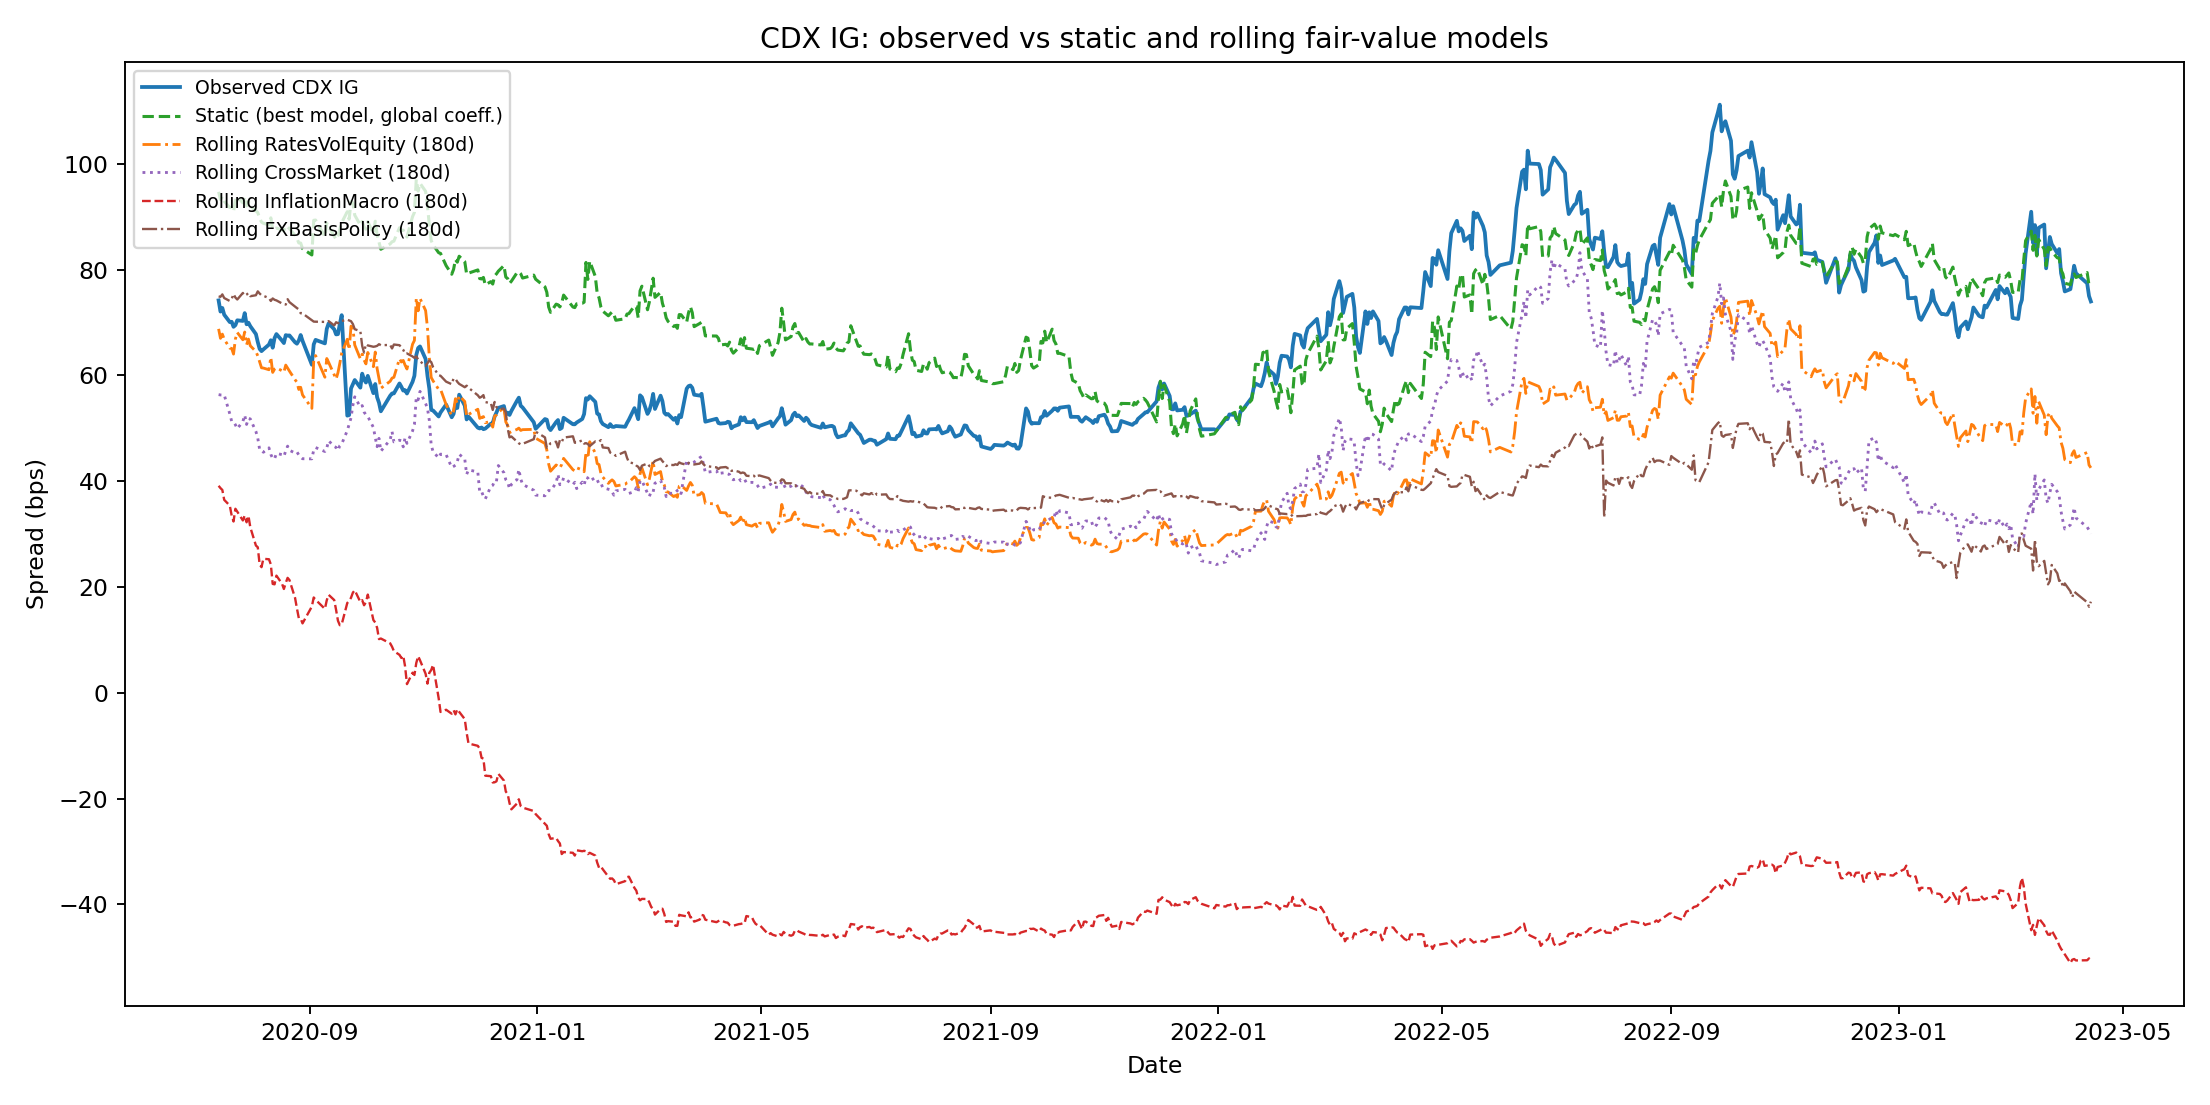
\includegraphics[width=\textwidth]{../../../output/figures/CDX_IG_fair_value_comparison.png}
  \caption{CDX IG observed spread vs static (global-coefficient) and rolling
    (180-day window) fair-value estimates for all candidate models with
    sufficient data.}
  \label{fig:fv_comparison}
\end{figure}
